\documentclass[12pt,a4paper]{article}
\usepackage[inner=1.5cm,outer=1.5cm,top=2.5cm,bottom=2.5cm]{geometry}
\usepackage{graphicx}
\graphicspath{ {./images/} }
\usepackage[english]{babel}
\usepackage{amsmath}
\usepackage{amssymb}
\numberwithin{equation}{subsection}
\usepackage{hyperref}
\usepackage[utf8]{inputenc}

\def\doubleunderline#1{\underline{\underline{#1}}}

\title{Statistics for Data Science \\
    Unit 3 Homework: Probability Theory}
\author{Brad Andersen \\
    W203 Section 4}
\date{January 23, 2019}

\begin{document}

\maketitle

\begin{enumerate}

% ----- Question 1: Gas Station Analytics ---------------------------------------------------

\item \textbf{Gas Station Analytics}
At a certain gas station, 40\% of customers use regular gas (event R), 35\% use mid-grade (event M), and 25\% use premium (event P).  Of the customers that use regular gas, 30\% fill their tanks (Event F).  Of the customers that use mid-grade gas, 60\% fill their tanks, while of those that use premium, 50\% fill their tanks.  Assume that each customer is drawn independently from the entire pool of customers.

\begin{table}[h]
\centering
\begin{tabular}{lll}
    $P(R) = 0.40$ & $P(M) = 0.35$ & $P(P) = 0.25$ \\
    $P(F|R) = 0.30$ & $P(F|M) = 0.60$ & $P(F|P) = 0.50$ \\
\end{tabular}
\caption{Known probabilities: Gas Station Analytics}
\end{table}

\begin{enumerate}
\item What is the probability that the next customer will request regular gas and fill the tank? \\ \\
$P(F|R) = \dfrac{P(F \cap R)}{P(R)}$ , therefore $P(F \cap R) = P(R) \times P(F|R)$ \\ \\
$P(F \cap R) = 0.40 \times 0.30$ \\ \\
$P(F \cap R) = 0.12$ \\ \\
Probability: $\doubleunderline{0.12}$ \\

\item What is the probability that the next customer will fill the tank? \\ \\
$(P(F|R) \times P(R)) + (P(F|M) \times P(M)) + (P(F|P) \times P(P))$ \\ \\
$(0.30 \times 0.40) + (0.60 \times 0.35) + (0.50 \times 0.25)$ \\ \\
$(0.12) + (0.21) + (0.125)$ \\ \\
Probability: $\doubleunderline{0.455}$ \\

\item Given that the next customer fills the tank, what is the conditional probability that they use regular gas? \\ \\
Let event T ("next customer fills tank") = 0.455. \\ \\
$P(R|T) = \dfrac{P(R \cap T)}{P(T)}$ , therefore $P(R|T) = \dfrac{P(T \cap R)}{P(T)}$ \\ \\
$P(R|T) = \dfrac{P(T|R) \times P(R)}{P(T)}$ \\ \\
$P(R|T) = \dfrac{0.30 \times 0.40}{0.455}$ \\ \\
$P(R|T) = \dfrac{0.12}{0.455}$ \\ \\
Probability: $\doubleunderline{0.264}$ \\

\end{enumerate}

% ----- Question 2: The Toy Bin -------------------------------------------------------------

\item \textbf{The Toy Bin}

 In a collection of toys, $1/2$ are red, $1/2$ are waterproof, and $1/3$ are cool. $1/4$ are red and waterproof.  $1/6$ are red and cool. $1/6$ are waterproof and cool. $1/6$ are neither red, waterproof, nor cool. Each toy has an equal chance of being selected.
 
\begin{table}[h]
\centering
\begin{tabular}{lll}
    $P(R)$ = red toy & $P(W)$ = waterproof toy & $P(C)$ = cool toy \\
\end{tabular}
\caption{Probability definitions: The Toy Bin}
\end{table}
 \begin{enumerate}
\item Draw an area diagram to represent these events. \\ \\
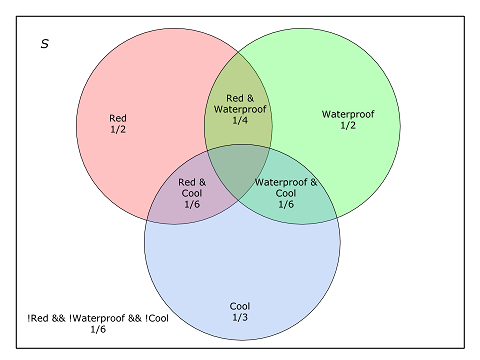
\includegraphics{images/unit3-q2_toybin-venn.png} \\ 

\item What is the probability of getting a red, waterproof, cool toy? \\ \\
Given that the probability of a toy being neither red nor waterproof nor cool is 1/6, the probability for the union of the probabilities of a toy being red or waterproof or cool is 1 - 1/6, or 5/6.  The value that must be calculated is the intersection of red, waterproof and cool in the Venn diagram, above. \\ \\
$\frac{5}{6} = P(R) + P(W) + P(C) - P(R \cap W) - P(R \cap C) - P(C \cap W) + P(R \cap W \cap C)$ \\ \\
$\frac{5}{6} = \frac{1}{2} + \frac{1}{2} + \frac{1}{3} - \frac{1}{4} - \frac{1}{6} - \frac{1}{6} + P(R \cap W \cap C)$ \\ \\
$\frac{5}{6} = \frac{3}{4} + P(R \cap W \cap C)$ \\ \\
$\frac{1}{12} = P(R \cap W \cap C)$ \\ \\
Probability: $\doubleunderline{\frac{1}{12}}$ \\

\item You pull out a toy at random and you observe only the color, noting that it is red.  Conditional on just this information, what is the probability that the toy is not cool? \\ \\
Probability = $P(R) - P(R \cap C)$ \\ \\
Probability = $\frac{1}{2} - \frac{1}{6}$ \\ \\
Probability = $\frac{6}{12} - \frac{2}{12}$ \\ \\
Probability = $\frac{4}{12} = \doubleunderline{\frac{1}{3}}$ \\

\item Given that a randomly selected toy is red or waterproof, what is the probability that it is cool? \\ \\
The following calculation assumes that "red or waterproof" does not mean that these are mutually exclusive events.  Rather, I am interpreting "red or waterproof" to mean that the selected toy can be both red and waterproof. \\ \\
Probability = $P(R \cap C) + P(W \cap C) - P(R \cap W \cap C)$ \\ \\
Probability = $\frac{1}{6} + \frac{1}{6} - \frac{1}{12}$ \\ \\
Probability = $\frac{3}{12} = \doubleunderline{\frac{1}{4}}$
\end{enumerate}
 
% ----- Question 3: The Overlap of Two Events -------------------------------------------

\item \textbf{On the Overlap of Two Events}
Suppose for events A and B, $P(A) = 1/2$, $P(B) = 2/3$, but we have no more information about the events.
 \begin{enumerate}
\item What are the maximum and minimum possible values for $P(A \cap B)$? \\ \\
The following diagram represents the intersections of $P(A)$ and $P(B)$ as probabilities in $S$: \\ \\
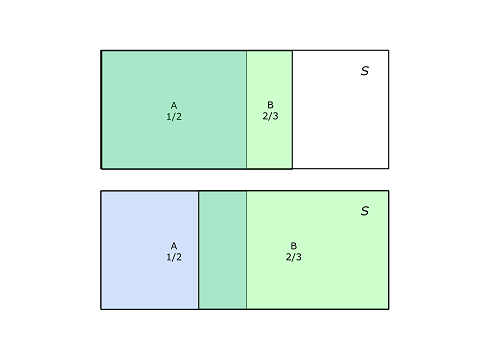
\includegraphics{images/unit3-q3_min-max-area.png}

Given that the probability of $S$ is 1, the maximum and minimum values for $P(A \cap B)$ are $\doubleunderline{\frac{1}{2}}$ and $\doubleunderline{\frac{1}{6}}$, respectively. \\ \\
\item What are the maximum and minimum possible values for $P(A|B)$? \\ \\
Given the definition of conditional probability: \\ \\ 
$P(A|B) = \dfrac{P(A \cap B)}{P(B)}$ \\ \\
Maximum and minimum values can be calculated as follows: \\ \\
Maximum: $P(A|B) = \dfrac{\frac{1}{2}}{\frac{2}{3}} = \doubleunderline{\frac{3}{4}}$ \\ \\
Minimum: $P(A|B) = \dfrac{\frac{1}{6}}{\frac{2}{3}} = \doubleunderline{\frac{1}{4}}$
\end{enumerate}

% ----- Question 4: Can't Please Everyone! ---------------------------------------------

\item \textbf{Can't Please Everyone!}
Among Berkeley students who have completed w203, $3/4$ like statistics.  Among Berkeley students who have not completed w203, only $1/4$ like statistics.  Assume that only 1 out of 100 Berkeley students completes w203.  Given that a Berkeley student likes statistics, what is the probability that they have completed w203? \\ \\
\begin{table}[h]
\centering
\begin{tabular}{lll}
    $P(C)$ = completed W203 & $P(N)$ = not completed W203 & $P(L)$ = like statistics \\
    $P(C)$ = 0.01 & $P(N)$ = 0.99 &
\end{tabular}
\caption{Probability definitions: Can't Please Everyone!}
\end{table} \\
$P(L|C) = \dfrac{P(L \cap C)}{P(C)}$ \\ \\
$P(L \cap C) = P(L|C) \times P(C)$ \\ \\
$P(L \cap C) = 0.75 \times 0.01$ \\ \\
$P(L \cap C) = 0.0075$ \\ \\
Probability = $\doubleunderline{0.0075}$

\end{enumerate}
\end{document}
